\subsection{Opening native research activities without simplifying the world}
\label{sec:native-activities-v6}

Free source and wiring are insufficient if consequential research inputs remain
hidden in a host coordinator. An opt-in activity graph now exposes native
research assignments, submission membership and actual paper bundles as typed
ports. It replaces four private annual-frame transports, not the researcher
world or its scientific phases. Assignments contain actual actor IDs, a freely
specified topic, focus, keywords and duration, project dates and submission
membership. A connected institution can author complete amendments in arbitrary
sandboxed Python or through an LLM mechanism. An explicit effect consumer
validates and applies them to actual researcher/project objects; collaboration,
submission and funding consume the resulting plans or actual archived paper IDs.
The host supplies no topic catalog, ranking or allocation policy for amendments.

Developer-authored native QA preserves six years of scientific state and every
researcher request against the original coordinator, for both one- and two-year
projects, including empty submission years. Connected free source changes real
research focus and permits a previously absent topic; another fixture changes
actual first-year submissions from four to three. Delayed amendments and cold
restart preserve effects, queues and causal events. Invalid IDs, mismatched
paper content, inconsistent dates, unsupported native value types and conflicting
writers are rejected before effect mutation. These are original-world software
tests with scripted corpus/retrieval/HTTP, not live-Qwen institutional discovery.
The native corpus/paper-production law and annual phase scheduler remain;
arbitrary new actor behavior or collaboration-pair semantics is not implied.

\subsection{Composed design-distribution gradients}
\label{sec:factorized-gradient-v6}

The score-function route no longer requires each policy action to be an entire
preassembled system. A caller supplies factors containing arbitrary source,
protocol, parameter and connection edits. Their selected edits compile as one
atomic transaction, allowing jointly changed interfaces that would be invalid
halfway through editing. Let $a_j$ be a component choice and $C_j(a_{<j})$ its
explicitly declared conditional support. The learned design policy is
\begin{align}
 q_\phi(a)&=\prod_j q_{\phi_j}(a_j\mid a_{<j},C_j),\\
 \nabla_\phi J(\phi)&=
 \mathbb{E}_{a\sim q_\phi,\xi}
 \left[(L(\mathrm{Sim}(S(a),\xi))-b)\nabla_\phi\log q_\phi(a)\right].
\end{align}
The complete original native forward, including responses to changed inputs
from the fixed-weight researcher LLM, supplies the cost. Backward differentiates
the exact joint design likelihood, not source strings, text tokens or the native
transition function. It thus avoids requiring a distorted differentiable forward
world, while remaining distinct from a faithful pathwise representation.

Conditional categorical and Bernoulli factors normalize within the declared
support; a forced singleton has zero score. A static preflight rejects the whole
invalid grammar, rather than silently dropping, repairing or remapping sampled
choices. Original latent assignments remain recorded even when they compile to
the same system. Any failed execution or replicate prevents the entire batch
update; it receives no invented cost and does not define a success-conditioned
objective. Baselines are fixed independently or leave-one-out for IID batches.
Equal-cost fixed-baseline samples can still produce nonzero score noise; a
nonzero gradient alone establishes no comparative advantage.

Exact enumerated expectation, score autograd and finite differences agree in
software tests. Eight complete six-year native QA worlds exercise both edge
states and both supplied protocol implementations, produce different actual
losses, update component logits and sample a subsequent composed design across
an interrupted/reopened campaign. Replies/corpus are scripted, not fresh Qwen
evidence. The supplied option vocabulary and finite preflight bound remain;
new source invention, continuous-coordinate differentiation and expected
native improvement do not follow from these checks.

\subsection{Objective-visible redesign within the same society}
\label{sec:persistent-session-v6}

A durable session connects previously separate interfaces:
\begin{center}
\small
actual interval $\to$ declared loss $\to$ external exact patch
$\to$ explicit adoption $\to$ subsequent interval.
\end{center}
Decision/review/delivery metrics are interval flows; resources and active authors
are end-boundary stocks. A proposer receives the exact current graph and prior
observations/adoptions. The controller neither invents a policy nor equates a
sequential before/after loss change with counterfactual superiority.

The staged request binds inspected whole-society and kernel hashes, loss, source
provenance and explicit memory/pending-message reconciliation. Exact-hash consent
only authorizes work; a separate saved-boundary worker performs the actual
transaction. A portable checkpoint, not an HTTP response, is authoritative for
adoption. If commit succeeds but its journal acknowledgement is interrupted,
reopening reconciles the actual migration receipt without repeating adoption.
The browser displays completion only after the saved original-rooted migration
chain and exact request identity verify. Historical reset-world v5 results and
the live continuity view are deliberately separate.

Independent review found and prompted fixes for two failure modes: inheriting
an acknowledged adoption in a foreign/rewound society, and overlooking unsaved
scientific fields through a partial stale-state serializer. Sessions now bind
the actual model/corpus/config/cache identity and preserve all acknowledged
receipts and observed event prefixes. Persistence and adoption share one complete
state capture, including RAG, extra actor state, resource/other native overlays,
RNG and replayable outputs. Scripted native QA covers repeated adoption, actual
future researcher inputs, explicit cancellation, write failure, cold restart
and commit-before-ack recovery. These are lifecycle guarantees, not a designer
improving its own algorithm or a demonstrated policy benefit.

\paragraph{A real failure beyond scripted lifecycle QA.}
The first actual continuation attempt completes year~1, external authorship,
browser consent and one durable installation, but stops during year~2 retrieval:
the portable restart has documents but no derived embedding index. Its passing
1,364-test regression did not cover that real-RAG condition. Independent read-only
audit retains all 21 raw files unchanged and distinguishes 24 checkpointed replies
from five partial-year replies; only the year~1 loss~0 is scored. The separate
correction rebuilds the derived index from the pinned corpus/cache without
advancing scientific RNG. Actual-RAG software regressions compare continuous
and cold-restarted researcher requests, scientific state and RNG. The failed
source/raw remain immutable; the corrected pilot starts from a new clean source,
with the same initial institution manifest explicitly reused rather than called
a newly invented design. This failure/retry is infrastructure evidence, not an
additional policy trial or optimizer replication.

An additional scripted interruption after real institution-code execution exposes
a second restart boundary: replies committed before an uncheckpointed year must
remain reusable. Prospective observations now pin their original ordered response
prefix. Only an already observed and adopted boundary may replay an intact
prefix with an additional verified response tail; new observation and adoption
remain strict. All other captured scientific state and RNG must still match.
Interrupted/restarted scientific state agrees with uninterrupted QA. The audit
also retains every physical code attempt: ambiguous repeated contexts or discarded
attempts do not count as additional committed scientific effects. Historical
observations lacking the new prefix proof are not retroactively relabelled.

\paragraph{Actual continuing-world execution.}
The separately pinned corrected pilot completes three native years in one society
with five Qwen researchers and two exact externally authored revisions. The
declared interval objective is $L=-A$, with no additional scientific-quality,
fairness or participation veto. Its loss path is $[0,-5,-5]$
(Figure~\ref{fig:native-society-v6}). After year~1, arbitrary Python supplies
one-year current research-plan amendments and an open-publication implementation;
actual native retrieval, papers, citations, review and funding remain. All five
real submissions are accepted in year~2 after 15 raw reviews. The next exact
request exposes this observed outcome and full source/graph history. Its revision
keeps the throughput policy, makes the complete plan the required primary input,
removes the old bypass and amendment edge, and preserves institution memory.
The graph changes from 14 nodes/18 edges to 15/21 and then 15/20: this is source,
protocol and authority rewiring, not a decorative extra node. Year~3 again has
five accepted papers and 15 reviews; the revision does not improve the count.

The same society's checkpoints and physical response database persist across both
adoptions. There are 130 actual replies (24,44,62 by interval), four recorded
source executions and no uncheckpointed replies or code contexts. Independent
read-only audit verifies all 36 raw files unchanged, exact authoring inputs,
migration/source/container receipts, actor continuity and eight re-extracted
interval metrics, without inference. Actual browser consent is pending until a
separate worker commits; final reload verifies both saved receipts with no
duplicate consent POST, browser errors or desktop/mobile overflow. External
Codex identity is self-reported, not authenticated and not Qwen authorship.
Sequential losses include calendar, project-history and model variation: this
is a completed online lifecycle, not a counterfactual benefit, held-out result,
scientifically useful invention or a designer improving its own algorithm.

\begin{figure}[ht]
\centering
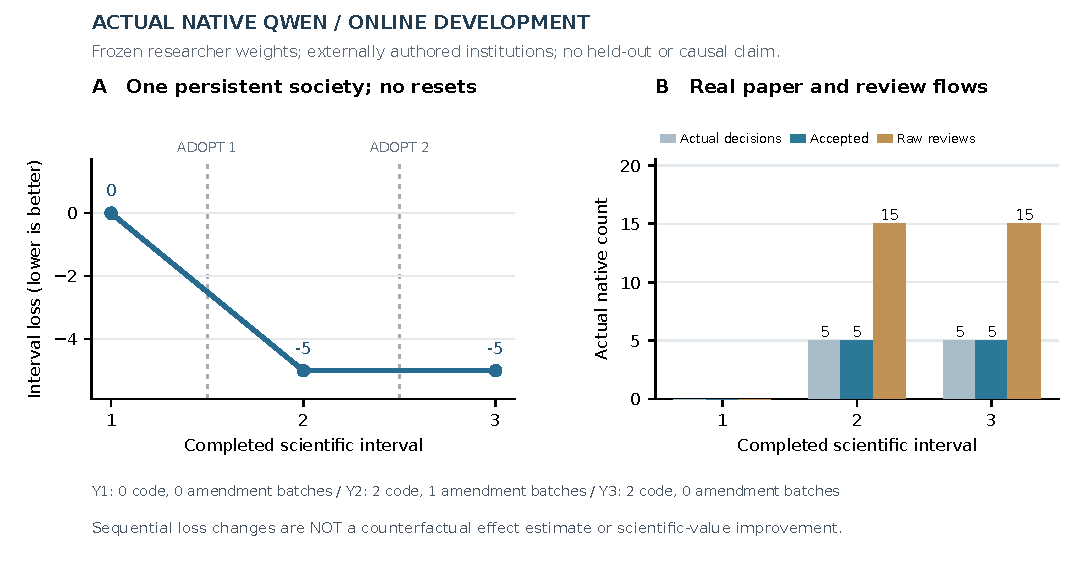
\includegraphics[width=\linewidth]{figures/native-society-v6.pdf}
\caption{Actual online redesign in one original native researcher society.
Two externally authored systems are installed at annual boundaries, without
resetting actors. The coarse count loss changes from~0 to~$-5$ and then ties.
Real paper/review flows are separately measured. The amendment-batch counter
falls to zero in year~3 because the new mechanism now supplies a complete primary
plan, not because its code or research effect disappears. This single trajectory
does not identify a causal institutional effect or scientific-value improvement.}
\label{fig:native-society-v6}
\end{figure}
